\documentclass{article}

% Language setting
% Replace `english' with e.g. `spanish' to change the document language
\usepackage[english]{babel}

% Set page size and margins
% Replace `letterpaper' with`a4paper' for UK/EU standard size
\usepackage[letterpaper,top=2cm,bottom=2cm,left=3cm,right=3cm,marginparwidth=1.75cm]{geometry}

% Useful packages
\usepackage{amsmath}
\usepackage{graphicx}
\graphicspath{ {./Figures/} }
\usepackage[colorlinks=true, allcolors=blue]{hyperref}

%\title{Your Paper}
%\author{You}

\begin{document}
\title{Xe129 - Rb87 Spin Exchange Optical Pumping dynamics}
\maketitle


% \begin{abstract}
% Your abstract.
% \end{abstract}

\section{Bloch equations}
The Block equation for the Xe spin are

\begin{align}
    \frac{d \mathbf{K}}{d t} &= -\gamma_{Xe}\left[\left( \mathbf{B}_0 + \mathbf{B}_d \cos{(\omega_{rf} t)}\right) + b_{KS} \mathbf{S}\right] \times\mathbf{K}  +\Gamma_{se} \left( \mathbf{S} - \mathbf{K}\right) - \Gamma_2 \hat{x}\left(\hat{x}\cdot \mathbf{K}\right)  - \Gamma_2 \hat{y}\left(\hat{y}\cdot \mathbf{K}\right) -  \Gamma_1 \hat{z}\left(\hat{z}\cdot \mathbf{K}\right)
\end{align}

Let us assume that $b_{KS} \mathbf{S}$ is part of the DC field $\mathbf{B}_0=B_0 \hat{z}$, that $\Gamma_{se} \left( \mathbf{S} - \mathbf{K}\right)=\left(\begin{array}{c}0\\0\\R_{se}\end{array}\right)$ and that the drive is $$\mathbf{B}_d \cos{(\omega_{rf} t)} =B_d \cos{(\omega_{rf} t)}\hat{x}$$ .

Thus, we end up with the next Bloch equation
\begin{align}
    \frac{d \mathbf{K}}{d t} &= -\gamma_{Xe}\left[\left( B_0\hat{z} + B_d \cos{(\omega_{rf} t)}\hat{x}\right) \right] \times\mathbf{K}  +R_{se}\hat{z} - \Gamma_2 \hat{x}\left(\hat{x}\cdot \mathbf{K}\right)  - \Gamma_2 \hat{y}\left(\hat{y}\cdot \mathbf{K}\right) -  \Gamma_1 \hat{z}\left(\hat{z}\cdot \mathbf{K}\right)\\
    &= -\gamma_{Xe} \begin{vmatrix}
        \hat{x}                     & \hat{y}       & \hat{z} \\
         B_d\cos{(\omega_{rf} t)}   & 0             & B_0  \\
         K_x                        & K_y           & K_z
    \end{vmatrix} + 
    \left(\begin{matrix}
         0  \\
         0  \\
         R_{se} 
    \end{matrix}\right) - 
    \left(\begin{matrix}
    \Gamma_2  &  0  &0\\
    0  &  \Gamma_2  &  0\\
    0  &  0  &  \Gamma_1 
    \end{matrix}\right)\cdot
    \left(\begin{matrix}
    K_x\\
    K_y\\
    K_z
    \end{matrix}\right)\\
    &= - \gamma_{Xe} 
    \left(\begin{matrix}
    -B_0 K_y\\
    B_0 K_x - B_d \cos{(\omega_{rf} t)} K_z\\
    B_d \cos{(\omega_{rf} t)} K_y
    \end{matrix}\right) + 
    \left(\begin{matrix}
         0  \\
         0  \\
         R_{se} 
    \end{matrix}\right) - 
    \left(\begin{matrix}
    \Gamma_2  &  0  &0\\
    0  &  \Gamma_2  &  0\\
    0  &  0  &  \Gamma_1 
    \end{matrix}\right)\cdot
    \left(\begin{matrix}
    K_x\\
    K_y\\
    K_z
    \end{matrix}\right)\\
    &=  
    \left(\begin{matrix}
    -\Gamma_2               &  \gamma_{Xe}B_0                        &  0                                    \\
    -\gamma_{Xe}B_0         &  -\Gamma_2                             &  \gamma_{Xe}B_d \cos{(\omega_{rf} t)} \\
    0                       &  -\gamma_{Xe}B_d \cos{(\omega_{rf} t)} &  -\Gamma_1 
    \end{matrix}\right)\cdot
    \left(\begin{matrix}
    K_x\\
    K_y\\
    K_z
    \end{matrix}\right) + 
    \left(\begin{matrix}
         0  \\
         0  \\
         R_{se} 
    \end{matrix}\right)\\
    &=  
    \left(\begin{matrix}
    -\Gamma_2               &  \omega_0                        &  0                              \\
    -\omega_0               &  -\Gamma_2                       &  \Omega_d \cos{(\omega_{rf} t)} \\
    0                       &  -\Omega_d \cos{(\omega_{rf} t)} &  -\Gamma_1 
    \end{matrix}\right)\cdot
    \left(\begin{matrix}
    K_x\\
    K_y\\
    K_z
    \end{matrix}\right) + 
    \left(\begin{matrix}
         0  \\
         0  \\
         R_{se} 
    \end{matrix}\right)
\end{align}

Finally, the Xe NMR dynamics can be described by the next Bloch equations

\begin{align}
    \left(\begin{matrix}
    \dot{K_x}\\
    \dot{K_y}\\
    \dot{K_z}
    \end{matrix}\right)
    &=  
    \left(\begin{matrix}
    -\Gamma_2               &  \omega_0                        &  0                              \\
    -\omega_0               &  -\Gamma_2                       &  \Omega_d \cos{(\omega_{rf} t)} \\
    0                       &  -\Omega_d \cos{(\omega_{rf} t)} &  -\Gamma_1 
    \end{matrix}\right)\cdot
    \left(\begin{matrix}
    K_x\\
    K_y\\
    K_z
    \end{matrix}\right) + 
    \left(\begin{matrix}
         0  \\
         0  \\
         R_{se} 
    \end{matrix}\right)
\end{align}


Now, let us move to the rotating frame (frame of Xe) using the next transformation

\begin{align}
    \left(\begin{array}{c}
        \tilde{K}_{x}\\
        \tilde{K}_{y}\\
        \tilde{K}_{z}
    \end{array}\right)	&=\left(\begin{array}{ccc}
        \cos(\omega_{0}t) & -\sin(\omega_{0}t) & 0\\
        \sin(\omega_{0}t) & \cos(\omega_{0}t) & 0\\
        0 & 0 & 1
    \end{array}\right)\left(\begin{array}{c}
        K_{x}\\
        K_{y}\\
        K_{z}
    \end{array}\right)\\
    \left(\begin{array}{c}
        K_{x}\\
        K_{y}\\
        K_{z}
    \end{array}\right)	&=\left(\begin{array}{ccc}
        \cos(\omega_{0}t) & \sin(\omega_{0}t) & 0\\
        -\sin(\omega_{0}t) & \cos(\omega_{0}t) & 0\\
        0 & 0 & 1
    \end{array}\right)\left(\begin{array}{c}
        \tilde{K}_{x}\\
        \tilde{K}_{y}\\
        \tilde{K}_{z}
    \end{array}\right)
\end{align}

Also, the derivative with respect to time of the transformation is
\begin{align}
    \left(\begin{array}{c}
        \dot{K_{x}}\\
        \dot{K_{y}}\\
        \dot{K_{z}}
    \end{array}\right)	&=\frac{d}{dt}\left[\left(\begin{array}{ccc}
        \cos(\omega_{0}t) & \sin(\omega_{0}t) & 0\\
        -\sin(\omega_{0}t) & \cos(\omega_{0}t) & 0\\
        0 & 0 & 1
    \end{array}\right)\left(\begin{array}{c}
        \tilde{K}_{x}\\
        \tilde{K}_{y}\\
        \tilde{K}_{z}
    \end{array}\right)\right]\\ 
    &=\frac{d}{dt}\left(\begin{array}{ccc}
        \cos(\omega_{0}t) & \sin(\omega_{0}t) & 0\\
        -\sin(\omega_{0}t) & \cos(\omega_{0}t) & 0\\
        0 & 0 & 1
    \end{array}\right)\left(\begin{array}{c}
        \tilde{K}_{x}\\
        \tilde{K}_{y}\\
        \tilde{K}_{z}
    \end{array}\right) + 
    \left(\begin{array}{ccc}
        \cos(\omega_{0}t) & \sin(\omega_{0}t) & 0\\
        -\sin(\omega_{0}t) & \cos(\omega_{0}t) & 0\\
        0 & 0 & 1
    \end{array}\right)
    \frac{d}{dt}\left(\begin{array}{c}
        \tilde{K}_{x}\\
        \tilde{K}_{y}\\
        \tilde{K}_{z}
    \end{array}\right)\\
    &=\omega_{0}\left(\begin{array}{ccc}
        -\sin(\omega_{0}t) & \cos(\omega_{0}t) & 0\\
        -\cos(\omega_{0}t) & -\sin(\omega_{0}t) & 0\\
        0 & 0 & 0
    \end{array}\right)
    \left(\begin{array}{c}
        \tilde{K}_{x}\\
        \tilde{K}_{y}\\
        \tilde{K}_{z}
    \end{array}\right) + 
    \left(\begin{array}{ccc}
        \cos(\omega_{0}t) & \sin(\omega_{0}t) & 0\\
        -\sin(\omega_{0}t) & \cos(\omega_{0}t) & 0\\
        0 & 0 & 1
    \end{array}\right)
    \frac{d}{dt}\left(\begin{array}{c}
        \tilde{K}_{x}\\
        \tilde{K}_{y}\\
        \tilde{K}_{z}
    \end{array}\right)
\end{align}



The Bloch equations transform as follows

\begin{align}
    \omega_{0}\left(\begin{array}{ccc}
        -\sin(\omega_{0}t) & \cos(\omega_{0}t) & 0\\
        -\cos(\omega_{0}t) & -\sin(\omega_{0}t) & 0\\
        0 & 0 & 0
    \end{array}\right)
    \left(\begin{array}{c}
        \tilde{K}_{x}\\
        \tilde{K}_{y}\\
        \tilde{K}_{z}
    \end{array}\right) + 
    \left(\begin{array}{ccc}
        \cos(\omega_{0}t) & \sin(\omega_{0}t) & 0\\
        -\sin(\omega_{0}t) & \cos(\omega_{0}t) & 0\\
        0 & 0 & 1
    \end{array}\right)
    \frac{d}{dt}\left(\begin{array}{c}
        \tilde{K}_{x}\\
        \tilde{K}_{y}\\
        \tilde{K}_{z}
    \end{array}\right)
    &=\\ 
    \left(\begin{matrix}
    -\Gamma_2               &  \omega_0                        &  0                              \\
    -\omega_0               &  -\Gamma_2                       &  \Omega_d \cos{(\omega_{rf} t)} \\
    0                       &  -\Omega_d \cos{(\omega_{rf} t)} &  -\Gamma_1 
    \end{matrix}\right)\cdot
    \left(\begin{array}{ccc}
        \cos(\omega_{0}t) & \sin(\omega_{0}t) & 0\\
        -\sin(\omega_{0}t) & \cos(\omega_{0}t) & 0\\
        0 & 0 & 1
    \end{array}\right)
    \left(\begin{array}{c}
        \tilde{K}_{x}\\
        \tilde{K}_{y}\\
        \tilde{K}_{z}
    \end{array}\right) &+ 
    \left(\begin{matrix}
         0  \\
         0  \\
         R_{se} 
    \end{matrix}\right)\\
    % new line
    \omega_{0}
    \left(\begin{array}{ccc}
        \cos(\omega_{0}t) & -\sin(\omega_{0}t) & 0\\
        \sin(\omega_{0}t) & \cos(\omega_{0}t) & 0\\
        0 & 0 & 1
    \end{array}\right)
    \left(\begin{array}{ccc}
        -\sin(\omega_{0}t) & \cos(\omega_{0}t) & 0\\
        -\cos(\omega_{0}t) & -\sin(\omega_{0}t) & 0\\
        0 & 0 & 0
    \end{array}\right)
    \left(\begin{array}{c}
        \tilde{K}_{x}\\
        \tilde{K}_{y}\\
        \tilde{K}_{z}
    \end{array}\right) + 
    \frac{d}{dt}\left(\begin{array}{c}
        \tilde{K}_{x}\\
        \tilde{K}_{y}\\
        \tilde{K}_{z}
    \end{array}\right)
    &=\\ 
    \left(\begin{array}{ccc}
        \cos(\omega_{0}t) & -\sin(\omega_{0}t) & 0\\
        \sin(\omega_{0}t) & \cos(\omega_{0}t) & 0\\
        0 & 0 & 1
    \end{array}\right)
    \left(\begin{matrix}
    -\Gamma_2               &  \omega_0                        &  0                              \\
    -\omega_0               &  -\Gamma_2                       &  \Omega_d \cos{(\omega_{rf} t)} \\
    0                       &  -\Omega_d \cos{(\omega_{rf} t)} &  -\Gamma_1 
    \end{matrix}\right)
    \left(\begin{array}{ccc}
        \cos(\omega_{0}t) & \sin(\omega_{0}t) & 0\\
        -\sin(\omega_{0}t) & \cos(\omega_{0}t) & 0\\
        0 & 0 & 1
    \end{array}\right)
    \left(\begin{array}{c}
        \tilde{K}_{x}\\
        \tilde{K}_{y}\\
        \tilde{K}_{z}
    \end{array}\right) &+ 
    \left(\begin{matrix}
         0  \\
         0  \\
         R_{se} 
    \end{matrix}\right)
\end{align}

Let us compute it separately term by term

\begin{align}
    \omega_{0}
    \left(\begin{array}{ccc}
        \cos(\omega_{0}t) & -\sin(\omega_{0}t) & 0\\
        \sin(\omega_{0}t) & \cos(\omega_{0}t) & 0\\
        0 & 0 & 1
    \end{array}\right)
    \left(\begin{array}{ccc}
        -\sin(\omega_{0}t) & \cos(\omega_{0}t) & 0\\
        -\cos(\omega_{0}t) & -\sin(\omega_{0}t) & 0\\
        0 & 0 & 0
    \end{array}\right)
    \left(\begin{array}{c}
        \tilde{K}_{x}\\
        \tilde{K}_{y}\\
        \tilde{K}_{z}
    \end{array}\right)&= 
    \omega_{0}
    \left(\begin{array}{ccc}
       0 & 1 & 0\\
       -1 & 0 & 0\\
        0 & 0 & 0
    \end{array}\right)
    \left(\begin{array}{c}
        \tilde{K}_{x}\\
        \tilde{K}_{y}\\
        \tilde{K}_{z}
    \end{array}\right)\\
    &=
    \omega_{0}
    \left(\begin{array}{c}
        \tilde{K}_{y}\\
        -\tilde{K}_{x}\\
        0
    \end{array}\right)
\end{align}

Also,

\begin{align}
    \left(\begin{array}{ccc}
        \cos(\omega_{0}t) & -\sin(\omega_{0}t) & 0\\
        \sin(\omega_{0}t) & \cos(\omega_{0}t) & 0\\
        0 & 0 & 1
    \end{array}\right)
    \left(\begin{matrix}
    -\Gamma_2               &  \omega_0                        &  0                              \\
    -\omega_0               &  -\Gamma_2                       &  \Omega_d \cos{(\omega_{rf} t)} \\
    0                       &  -\Omega_d \cos{(\omega_{rf} t)} &  -\Gamma_1 
    \end{matrix}\right)
    \left(\begin{array}{ccc}
        \cos(\omega_{0}t) & \sin(\omega_{0}t) & 0\\
        -\sin(\omega_{0}t) & \cos(\omega_{0}t) & 0\\
        0 & 0 & 1
    \end{array}\right) &=\\
    \left(\begin{array}{ccc}
        \cos(\omega_{0}t) & -\sin(\omega_{0}t) & 0\\
        \sin(\omega_{0}t) & \cos(\omega_{0}t) & 0\\
        0 & 0 & 1
    \end{array}\right)
    \left(\begin{matrix}
    -\Gamma_2 \cos(\omega_{0}t) -\omega_{0}\sin(\omega_{0}t) & -\Gamma_2 \sin(\omega_{0}t) +\omega_{0}\cos(\omega_{0}t)    &  0  \\
    -\omega_{0} \cos(\omega_{0}t) + \Gamma_2 \sin(\omega_{0}t)   &  -\omega_{0} \sin(\omega_{0}t) - \Gamma_2 \cos(\omega_{0}t)  &  \Omega_d \cos{(\omega_{rf} t)} \\ \Omega_d \cos{(\omega_{rf} t)}\sin(\omega_{0}t) &  -\Omega_d \cos{(\omega_{rf} t)}\cos(\omega_{0}t) &  -\Gamma_1 
    \end{matrix}\right) &=\\
    % last line
    \left(\begin{matrix}
    -\Gamma_2 & \omega_{0}    &  -\Omega_d \cos{(\omega_{rf} t)}\sin(\omega_{0}t) \\
    -\omega_{0} &  - \Gamma_2 &  \Omega_d \cos{(\omega_{rf} t)}\cos(\omega_{0}t) \\ \Omega_d \cos{(\omega_{rf} t)}\sin(\omega_{0}t) &  -\Omega_d \cos{(\omega_{rf} t)}\cos(\omega_{0}t) &  -\Gamma_1 
    \end{matrix}\right)
\end{align}

combining the terms together we get

\begin{align}
    \omega_{0}
    \left(\begin{array}{ccc}
       0 & 1 & 0\\
       -1 & 0 & 0\\
        0 & 0 & 0
    \end{array}\right)
    \left(\begin{array}{c}
        \tilde{K}_{x}\\
        \tilde{K}_{y}\\
        \tilde{K}_{z}
    \end{array}\right) + 
    \frac{d}{dt}\left(\begin{array}{c}
        \tilde{K}_{x}\\
        \tilde{K}_{y}\\
        \tilde{K}_{z}
    \end{array}\right)
    &=\\
   \left(\begin{matrix}
    -\Gamma_2 & \omega_{0}    &  -\Omega_d \cos{(\omega_{rf} t)}\sin(\omega_{0}t) \\
    -\omega_{0} &  - \Gamma_2 &  \Omega_d \cos{(\omega_{rf} t)}\cos(\omega_{0}t) \\ \Omega_d \cos{(\omega_{rf} t)}\sin(\omega_{0}t) &  -\Omega_d \cos{(\omega_{rf} t)}\cos(\omega_{0}t) &  -\Gamma_1 
    \end{matrix}\right)
    \left(\begin{array}{c}
        \tilde{K}_{x}\\
        \tilde{K}_{y}\\
        \tilde{K}_{z}
    \end{array}\right) &+ 
    \left(\begin{matrix}
         0  \\
         0  \\
         R_{se} 
    \end{matrix}\right)\\
    \frac{d}{dt}\left(\begin{array}{c}
        \tilde{K}_{x}\\
        \tilde{K}_{y}\\
        \tilde{K}_{z}
    \end{array}\right)
    &=\\
   \left(\begin{matrix}
    -\Gamma_2 & \omega_{0}    &  -\Omega_d \cos{(\omega_{rf} t)}\sin(\omega_{0}t) \\
    -\omega_{0} &  - \Gamma_2 &  \Omega_d \cos{(\omega_{rf} t)}\cos(\omega_{0}t) \\ \Omega_d \cos{(\omega_{rf} t)}\sin(\omega_{0}t) &  -\Omega_d \cos{(\omega_{rf} t)}\cos(\omega_{0}t) &  -\Gamma_1 
    \end{matrix}\right)
    \left(\begin{array}{c}
        \tilde{K}_{x}\\
        \tilde{K}_{y}\\
        \tilde{K}_{z}
    \end{array}\right) &+
    \left(\begin{array}{ccc}
       0 & -\omega_{0} & 0\\
       \omega_{0} & 0 & 0\\
        0 & 0 & 0
    \end{array}\right)
    \left(\begin{array}{c}
        \tilde{K}_{x}\\
        \tilde{K}_{y}\\
        \tilde{K}_{z}
    \end{array}\right)\\&+ 
    \left(\begin{matrix}
         0  \\
         0  \\
         R_{se} 
    \end{matrix}\right)
\end{align}

so finally

\begin{align}
    \frac{d}{dt}\left(\begin{array}{c}
        \tilde{K}_{x}\\
        \tilde{K}_{y}\\
        \tilde{K}_{z}
    \end{array}\right)
    &=
   \left(\begin{matrix}
    -\Gamma_2 & 0    &  -\Omega_d \cos{(\omega_{rf} t)}\sin(\omega_{0}t) \\
    0 &  - \Gamma_2 &  \Omega_d \cos{(\omega_{rf} t)}\cos(\omega_{0}t) \\ \Omega_d \cos{(\omega_{rf} t)}\sin(\omega_{0}t) &  -\Omega_d \cos{(\omega_{rf} t)}\cos(\omega_{0}t) &  -\Gamma_1 
    \end{matrix}\right)
    \left(\begin{array}{c}
        \tilde{K}_{x}\\
        \tilde{K}_{y}\\
        \tilde{K}_{z}
    \end{array}\right) + 
    \left(\begin{matrix}
         0  \\
         0  \\
         R_{se} 
    \end{matrix}\right)\\
\end{align}

Notice that in the case where we transfer to a different rotating frame of reference which rotates at some frequency $\omega_1$, then the Bloch equations would be a bit different after the transformation

\begin{align}
    \frac{d}{dt}\left(\begin{array}{c}
        \tilde{K}_{x}\\
        \tilde{K}_{y}\\
        \tilde{K}_{z}
    \end{array}\right)
    &=
   \left(\begin{matrix}
    -\Gamma_2 & \omega_0-\omega_1    &  -\Omega_d \cos{(\omega_{rf} t)}\sin(\omega_{1}t) \\
    -\left( \omega_0-\omega_1\right) &  - \Gamma_2 &  \Omega_d \cos{(\omega_{rf} t)}\cos(\omega_{1}t) \\ \Omega_d \cos{(\omega_{rf} t)}\sin(\omega_{1}t) &  -\Omega_d \cos{(\omega_{rf} t)}\cos(\omega_{1}t) &  -\Gamma_1 
    \end{matrix}\right)
    \left(\begin{array}{c}
        \tilde{K}_{x}\\
        \tilde{K}_{y}\\
        \tilde{K}_{z}
    \end{array}\right) + 
    \left(\begin{matrix}
         0  \\
         0  \\
         R_{se} 
    \end{matrix}\right)\\
\end{align}

Using trigonometric identities we can simplify the drive terms in the Bloch matrix

\begin{align}
    \Omega_d \cos{(\omega_{rf} t)}\sin(\omega_{1}t) &= \frac{\Omega_d}{2} \left(\sin(\left(\omega_{rf}+\omega_{1}\right)t)+\sin(\left(\omega_{rf}-\omega_{1}\right)t)\right)\\
    \Omega_d \cos{(\omega_{rf} t)}\cos(\omega_{1}t) &= \frac{\Omega_d}{2} \left(\cos(\left(\omega_{rf}-\omega_{1}\right)t)+\cos(\left(\omega_{rf}+\omega_{1}\right)t)\right)\\
\end{align}

assuming that $\omega_{rf} - \omega_{1} \ll 1$, then we can use the RWA which states that fast oscillations average out to zero

\begin{align}
    \Omega_d \cos{(\omega_{rf} t)}\sin(\omega_{1}t) &= \frac{\Omega_d}{2} \sin(2\omega_{rf}t)=0\\
    \Omega_d \cos{(\omega_{rf} t)}\cos(\omega_{1}t) &= \frac{\Omega_d}{2} \left(1+\cos(2\omega_{rf}t)\right)=\frac{\Omega_d}{2}\\
\end{align}

Then, the Bloch equations with the RWA are

\begin{align}
    \frac{d}{dt}\left(\begin{array}{c}
        \tilde{K}_{x}\\
        \tilde{K}_{y}\\
        \tilde{K}_{z}
    \end{array}\right)=
   \left(\begin{matrix}
    -\Gamma_2 & \omega_0-\omega_{rf}    &  0 \\
    -\left( \omega_0-\omega_{rf}\right) &  - \Gamma_2 &  \frac{\Omega_d}{2} \\ 0 &  -\frac{\Omega_d}{2}  &  -\Gamma_1 
    \end{matrix}\right)
    \left(\begin{array}{c}
        \tilde{K}_{x}\\
        \tilde{K}_{y}\\
        \tilde{K}_{z}
    \end{array}\right) + 
    \left(\begin{matrix}
         0  \\
         0  \\
         R_{se} 
    \end{matrix}\right)
\end{align}

Next, we add to our model The effective magnetic field the Xe particles fill which produced by the alkali atoms, $b_{KS}\mathbf{S}=b_{KS}S_z\hat{z}$ and also
some world rotation $\mathbf{\omega_r} = \omega_r\hat{z}$.

The modified equations are

\begin{align}
    \boxed{\frac{d}{dt}\left(\begin{array}{c}
        \tilde{K}_{x}\\
        \tilde{K}_{y}\\
        \tilde{K}_{z}
    \end{array}\right)=
   \left(\begin{matrix}
    -\Gamma_2 & M_{12}    &  0 \\
    M_{21} &  - \Gamma_2 &  \frac{\Omega_d}{2} \\ 0 &  -\frac{\Omega_d}{2}  &  -\Gamma_1 
    \end{matrix}\right)
    \left(\begin{array}{c}
        \tilde{K}_{x}\\
        \tilde{K}_{y}\\
        \tilde{K}_{z}
    \end{array}\right) + 
    \left(\begin{matrix}
         0  \\
         0  \\
         R_{se} 
    \end{matrix}\right)}\label{eq:Bloch_equations}
\end{align}

where $M_{21}=-M_{12}$ and
\begin{align}
    M_{12} &= \omega_{0}+\gamma_{Xe}b_{KS}S_z+\omega_r-\omega_{rf}\\
        &= \gamma_{Xe}B_0+\gamma_{Xe}b_{KS}S_z+\omega_r-\omega_{rf}\\
\end{align}

Next, let us find the steady state solution of the Bloch equations in the rotating frame with drive in $\hat{x}$ with the RWA

\begin{align}
    \left(\begin{matrix}
    \Gamma_2 & -M_{12}    &  0 \\
    M_{12} &   \Gamma_2 &  -\frac{\Omega_d}{2} \\ 0 &  \frac{\Omega_d}{2}  &  \Gamma_1 
    \end{matrix}\right)
    \left(\begin{array}{c}
        \tilde{K}_{x}\\
        \tilde{K}_{y}\\
        \tilde{K}_{z}
    \end{array}\right) = 
    \left(\begin{matrix}
         0  \\
         0  \\
         R_{se} 
    \end{matrix}\right)
\end{align}

\begin{align}
    \left(\begin{array}{c}
        \Gamma_2\tilde{K}_{x} - M_{12}\tilde{K}_{y}\\
        M_{12}\tilde{K}_{x}+\Gamma_2\tilde{K}_{y}-\frac{\Omega_d}{2}\tilde{K}_{z}\\
        \frac{\Omega_d}{2}\tilde{K}_{y}+\Gamma_1\tilde{K}_{z}
    \end{array}\right)&=
    \left(\begin{array}{c}
        0\\
        0\\
        R_{se} 
    \end{array}\right)
\end{align}

\begin{align}
    \tilde{K}_{x} &= \frac{M_{12}}{\Gamma_2}\tilde{K}_{y}\\
\end{align}

\begin{align}
    \left(\begin{array}{c}
        \frac{M_{12}^2+\Gamma_2^2}{\Gamma_2}\tilde{K}_{y}-\frac{\Omega_d}{2}\tilde{K}_{z}\\
        \frac{\Omega_d}{2}\tilde{K}_{y}+\Gamma_1\tilde{K}_{z}
    \end{array}\right)&=
    \left(\begin{array}{c}
        0\\
        R_{se} 
    \end{array}\right)\\
    \left(\begin{array}{c}
        \left(1 + \left(M_{12}/\Gamma_2\right)^2\right)\Gamma_2\tilde{K}_{y}-\frac{\Omega_d}{2}\tilde{K}_{z}\\
        \frac{\Omega_d}{2}\tilde{K}_{y}+\Gamma_1\tilde{K}_{z}
    \end{array}\right)&=
    \left(\begin{array}{c}
        0\\
        R_{se} 
    \end{array}\right)
\end{align}


\begin{align}
   \left(1 + \left(M_{12}/\Gamma_2\right)^2\right)\Gamma_2 \tilde{K}_{y} &=  \frac{\Omega_d}{2}\tilde{K}_{z}\\
    \tilde{K}_{y} &=  \frac{\frac{\Omega_d}{2}}{\left(1 + \left(M_{12}/\Gamma_2\right)^2\right)\Gamma_2}\tilde{K}_{z}\\
\end{align}

\begin{align}
    \frac{\Omega_d}{2}\tilde{K}_{y} + \Gamma_1 \tilde{K}_{z} &= R_{se}\\
    \frac{\Omega_d}{2}\frac{\frac{\Omega_d}{2}}{\left(1 + \left(M_{12}/\Gamma_2\right)^2\right)\Gamma_2}\tilde{K}_{z} + \Gamma_1 \tilde{K}_{z} &= R_{se}\\
    \frac{\frac{\Omega_d^2}{4} + \left(1 + \left(M_{12}/\Gamma_2\right)^2\right)\Gamma_2\Gamma_1}{\left(1 + \left(M_{12}/\Gamma_2\right)^2\right)\Gamma_2} \tilde{K}_{z} &= R_{se}\\
    \frac{\frac{\Omega_d^2}{4\Gamma_2\Gamma_1} + \left(1 + \left(M_{12}/\Gamma_2\right)^2\right)}{\left(1 + \left(M_{12}/\Gamma_2\right)^2\right)/\Gamma_1} \tilde{K}_{z} &= R_{se}\\
     \tilde{K}_{z} &= \frac{R_{se}}{\Gamma_1} \frac{\left(1 + \left(M_{12}/\Gamma_2\right)^2\right)}{\frac{\Omega_d^2}{4\Gamma_2\Gamma_1} + \left(1 + \left(M_{12}/\Gamma_2\right)^2\right)}
\end{align}

\begin{align}
    \tilde{K}_{y} &=  \frac{\Omega_d}{2\Gamma_2}\frac{R_{se}}{\Gamma_1} \frac{1}{\frac{\Omega_d^2}{4\Gamma_2\Gamma_1} + \left(1 + \left(M_{12}/\Gamma_2\right)^2\right)}
\end{align}

\begin{align}
    \tilde{K}_{x} &= \frac{M_{12}}{\Gamma_2}\frac{\Omega_d}{2\Gamma_2}\frac{R_{se}}{\Gamma_1} \frac{1}{\frac{\Omega_d^2}{4\Gamma_2\Gamma_1} + \left(1 + \left(M_{12}/\Gamma_2\right)^2\right)}
\end{align}
    
Finally, the solution to the Bloch equation (eq.(\ref{eq:Bloch_equations})) is

\begin{align}
    \boxed{\left(\begin{array}{c}
        \tilde{K}_{x}\\
        \tilde{K}_{y}\\
        \tilde{K}_{z} 
    \end{array}\right)=
    \frac{\frac{R_{se}}{\Gamma_1}}{\frac{\Omega_d^2}{4\Gamma_2\Gamma_1} + \left(1 + \left(M_{12}/\Gamma_2\right)^2\right)}
    \left(\begin{array}{c}
      \frac{M_{12}}{\Gamma_2}\frac{\Omega_d}{2\Gamma_2} \\
       \frac{\Omega_d}{2\Gamma_2}\\
         \left(1 + \left(M_{12}/\Gamma_2\right)^2\right)
    \end{array}\right)}\label{eq:Bloch_solution}
\end{align}

In the case where $M_{12}=0$ we get

\begin{align}
    \left(\begin{array}{c}
        \tilde{K}_{x}\\
        \tilde{K}_{y}\\
        \tilde{K}_{z} 
    \end{array}\right)=
    \frac{\frac{R_{se}}{\Gamma_1}}{1+\frac{\Omega_d^2}{4\Gamma_2\Gamma_1}}
    \left(\begin{array}{c}
      0 \\
       \frac{\Omega_d}{2\Gamma_2}\\
         1
    \end{array}\right)
\end{align}

Recall that we measure the transverse spin polarization. Let us compute the optimal drive amplitude for maximal $\tilde{K}_y$ polarization

\begin{align}
    \frac{d\tilde{K}_{y}}{d \Omega_d} = \frac{R_{se}}{2\Gamma_2\Gamma_1}\frac{1}{1+\frac{\Omega_d^2}{4\Gamma_2\Gamma_1}} - \frac{R_{se}}{2\Gamma_2\Gamma_1}\frac{\Omega_d^2}{\Gamma_2\Gamma_1} \frac{1}{\left(1+\frac{\Omega_d^2}{4\Gamma_2\Gamma_1}\right)^2}=0
\end{align}

we get the next optimal drive amplitude $$\Omega_d^{\text{optimal}} = \sqrt{\frac{4\Gamma_2\Gamma_1}{3}}$$

for the optimal drive, the $\hat{z}$ polarization would be
$$\tilde{K}_{z} = \frac{3R_{se}}{4\Gamma_1}$$

We can make the same calculation in the case where $M_{12}\neq 0$

\begin{align}
    \frac{d\tilde{K}_{y}}{d \Omega_d} = \frac{R_{se}}{2\Gamma_2\Gamma_1}\frac{1}{\frac{\Omega_d^2}{4\Gamma_2\Gamma_1} + \left(1 + \left(M_{12}/\Gamma_2\right)^2\right)} - \frac{R_{se}}{2\Gamma_2\Gamma_1}\frac{\Omega_d^2}{\Gamma_2\Gamma_1} \frac{1}{\left(\frac{\Omega_d^2}{4\Gamma_2\Gamma_1} + \left(1 + \left(M_{12}/\Gamma_2\right)^2\right)\right)^2}=0
\end{align}

in that case the optimal drive amplitude is

\begin{align}
    \Omega_d^{\text{optimal}} =\sqrt{\frac{4\Gamma_2\Gamma_1}{3}}\sqrt{1 + \left(M_{12}/\Gamma_2\right)^2}\label{eq:optimal_drive}
\end{align}


Just for sports we can also solve the case of drive in $\hat{y}$, the Bloch equations in that case are

\begin{align}
    \boxed{\frac{d}{dt}\left(\begin{array}{c}
        \tilde{K}_{x}\\
        \tilde{K}_{y}\\
        \tilde{K}_{z}
    \end{array}\right)=
   \left(\begin{matrix}
    -\Gamma_2 & M_{12}    &  -\frac{\Omega_d}{2} \\
    M_{21} &  - \Gamma_2 &  0 \\ \frac{\Omega_d}{2} &   0 &  -\Gamma_1 
    \end{matrix}\right)
    \left(\begin{array}{c}
        \tilde{K}_{x}\\
        \tilde{K}_{y}\\
        \tilde{K}_{z}
    \end{array}\right) + 
    \left(\begin{matrix}
         0  \\
         0  \\
         R_{se} 
    \end{matrix}\right)}\label{eq:Bloch_equations_y_drive}
\end{align}

then the steady state solution would be

\begin{align}
    \left(\begin{array}{c}
        \Gamma_2\tilde{K}_{x} - M_{12}\tilde{K}_{y} + \frac{\Omega_d}{2}\tilde{K}_{z}\\
        M_{12}\tilde{K}_{x}+\Gamma_2\tilde{K}_{y}\\
        -\frac{\Omega_d}{2}\tilde{K}_{x}+\Gamma_1\tilde{K}_{z}
    \end{array}\right)&=
    \left(\begin{array}{c}
        0\\
        0\\
        R_{se} 
    \end{array}\right)
\end{align}


$$\tilde{K}_y = - \frac{M_{12}}{\Gamma_2}\tilde{K}_x$$

\begin{align}
     \left(\begin{array}{c}
        \frac{\Gamma_2^2 + M_{12}^2}{\Gamma_2}\tilde{K}_{x} + \frac{\Omega_d}{2}\tilde{K}_{z}\\
        -\frac{\Omega_d}{2}\tilde{K}_{x}+\Gamma_1\tilde{K}_{z}
    \end{array}\right)&=
    \left(\begin{array}{c}
        0\\
        R_{se} 
    \end{array}\right)\\
    \left(\begin{array}{c}
        \left(1 + \left(M_{12}/\Gamma_2\right)^2\right)\Gamma_2\tilde{K}_{x} + \frac{\Omega_d}{2}\tilde{K}_{z}\\
        -\frac{\Omega_d}{2}\tilde{K}_{x}+\Gamma_1\tilde{K}_{z}
    \end{array}\right)&=
    \left(\begin{array}{c}
        0\\
        R_{se} 
    \end{array}\right)
\end{align}

$$\tilde{K}_{x} = -\frac{\Omega_d}{2}\frac{1}{\left(1 + \left(M_{12}/\Gamma_2\right)^2\right)\Gamma_2}\tilde{K}_{z}$$

$$\tilde{K}_{z} = \frac{R_{se}}{\Gamma_1} \frac{\left(1 + \left(M_{12}/\Gamma_2\right)^2\right)}{\frac{\Omega_d^2}{4\Gamma_2\Gamma_1} + \left(1 + \left(M_{12}/\Gamma_2\right)^2\right)} $$

so finally,

\begin{align}
    \boxed{\left(\begin{array}{c}
        \tilde{K}_{x}\\
        \tilde{K}_{y}\\
        \tilde{K}_{z} 
    \end{array}\right)=
    \frac{\frac{R_{se}}{\Gamma_1}}{\frac{\Omega_d^2}{4\Gamma_2\Gamma_1} + \left(1 + \left(M_{12}/\Gamma_2\right)^2\right)}
    \left(\begin{array}{c}
    -\frac{\Omega_d}{2\Gamma_2}\\
      \frac{M_{12}}{\Gamma_2}\frac{\Omega_d}{2\Gamma_2} \\
         \left(1 + \left(M_{12}/\Gamma_2\right)^2\right)
    \end{array}\right)}\label{eq:Bloch_solution_y_drive}
\end{align}



\section{NMR Gyroscope (NMRG)}
Using the Xenon NMR model (the Bloch equations) we can implement a gyroscope which measures rotation along the primary axis of the system (in the case above: $\hat{z}$). 
Following Walker's notation in \cite{walker2016spin}, we break the spin dynamics into two components, parallel and perpendicular to the primary axis $\hat{z}$  $$\mathbf{K}=K_z\hat{z}+\mathbf{K}_{\perp}$$

describing $\mathbf{K}_{\perp}$ using a phasor notation
$$K_{+} = K_x + iK_y = K_{\perp}e^{-i\phi}$$
where $$K_{\perp}=\sqrt{K_x^2+K_y^2}\quad, \quad \phi=\arctan{\left(\frac{K_y}{K_x}\right)}$$

% Solving for the perpendicular polarization in the rotating frame we get

% \begin{align}
%     \frac{d\tilde{K}_{+}}{dt} &= \frac{d\tilde{K}_{x}}{dt}+i\frac{d\tilde{K}_{y}}{dt}\\
%     &=-\Gamma_2 \tilde{K}_x + M_{12} \tilde{K}_y - \frac{\Omega_d}{2} \tilde{K}_z \\&- iM_{12} \tilde{K}_{x} - i\Gamma_2\tilde{K}_{y}\\
% \end{align}


Now, if we solve for $\phi$ in the rotating frame of the drive, from eq.(\ref{eq:Bloch_solution_y_drive}) we get

\begin{align}
    \phi = \arctan{\left(\frac{\tilde{K}_y}{\tilde{K}_x}\right)}=\arctan{\left(-\frac{M_{12}}{\Gamma_2}\right)}
\end{align}

for small phase, where $M_{12}\ll 1$ the phase can be approximated with its zeroth order Taylor expansion $$\phi= -\frac{M_{12}}{\Gamma_2}$$

unfolding $M_{12}$ we get
$$\phi= -\frac{\gamma_{Xe}B_0}{\Gamma_2}-\frac{\gamma_{Xe}b_{KS}S_z}{\Gamma_2}-\frac{\omega_r}{\Gamma_2}+\frac{\omega_{rf}}{\Gamma_2}$$

In a real life NMR system we would also have some magnetic noise in the primary axis $\gamma_{Xe} B_{noise}$, so the phase would be
$$\phi= -\frac{\gamma_{Xe}B_0}{\Gamma_2}-\frac{\gamma_{Xe}B_{noise}}{\Gamma_2}-\frac{\gamma_{Xe}b_{KS}S_z}{\Gamma_2}-\frac{\omega_r}{\Gamma_2}+\frac{\omega_{rf}}{\Gamma_2}$$

all these parameters could in general be time dependent. Notice that in the phase equation we have two unknown parameters: fluctuations of the magnetic field $B_{noise}$ and the world rotation $\omega_r$. In order two extract the world rotation from the phase measurements we need to introduce another specie.  


\subsection{Dual species open-loop NMRG scheme}
Having a system with two species, Xe129 and Xe131, we can compute the world rotation as follows

\begin{align}
    \phi_{129} &= -\frac{\gamma^{129}_{Xe}B_0}{\Gamma_2^{129}}-\frac{\gamma^{129}_{Xe}B_{noise}}{\Gamma_2^{129}}-\frac{\gamma^{129}_{Xe}b_{KS}S_z}{\Gamma_2^{129}}-\frac{\omega_r}{\Gamma_2^{129}}+\frac{\omega^{129}_{rf}}{\Gamma_2^{129}}\\
    \phi_{131} &= -\frac{\gamma^{131}_{Xe}B_0}{\Gamma_2^{131}}-\frac{\gamma^{131}_{Xe}B_{noise}}{\Gamma_2^{131}}-\frac{\gamma^{131}_{Xe}b_{KS}S_z}{\Gamma_2^{131}}-\frac{\omega_r}{\Gamma_2^{131}}+\frac{\omega^{131}_{rf}}{\Gamma_2^{131}}
\end{align}

Then, subtracting the two equations we get

\begin{align}
    \frac{1}{\gamma^{129}_{Xe}}\left(\phi_{129}\Gamma_2^{129}-\omega^{129}_{rf}\right) - \frac{1}{\gamma^{131}_{Xe}}\left(\phi_{131}\Gamma_2^{131}-\omega^{131}_{rf}\right) &= \omega_r \left(\frac{1}{\gamma^{131}_{Xe}} - \frac{1}{\gamma^{129}_{Xe}}\right)
\end{align}

and finally the world rotation in an open-loop setting is given by 

\begin{align}
    \omega_r &= \left[\frac{ \gamma^{129}_{Xe} \gamma^{131}_{Xe} }{\gamma^{129}_{Xe} - \gamma^{131}_{Xe}}\right]\left[\frac{1}{\gamma^{129}_{Xe}}\left(\phi_{129}\Gamma_2^{129}-\omega^{129}_{rf}\right) - \frac{1}{\gamma^{131}_{Xe}}\left(\phi_{131}\Gamma_2^{131}-\omega^{131}_{rf}\right)\right]\label{eq:open-loop-world-rotation}
\end{align}

A scheme of such dual species open-loop system is illustrated in Fig.(\ref{fig:open_loop_scheme}).

\begin{figure}[h]
\centering
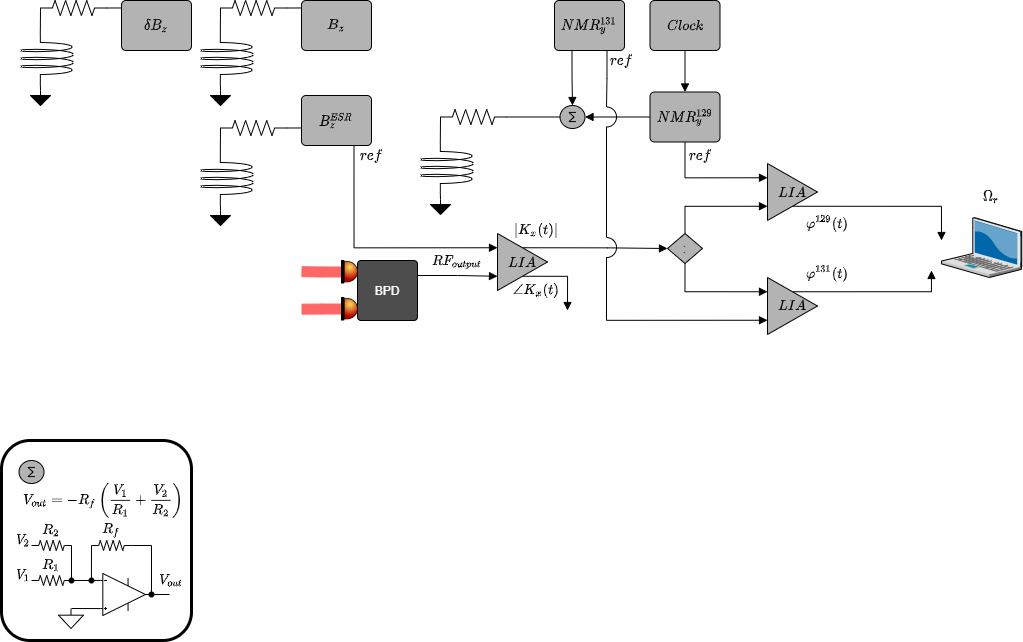
\includegraphics[width=0.9\textwidth]{Theory/Figures/NMRG_open_loop_scheme.png}
\caption{Dual species NMRG open-loop scheme. The Alkali signal is measured in a Balanced Photo detector (BPD) which is then inserted into a Lock-in amplifier (LIA) with a parametric modulation ($B^{ESR}_t$) reference. The amplitude extracted from the LIA channel is the Xenon dynamic which is then been splitted and inserted into two more LIAs with two NMR drive references ($NMR^{129}_y\,NMR^{131}_y$) one for each Xenon. The two phases extracted from the LIAs are the two Xenon phase differences from their drive signals. These phase signals can be used to compute the world rotation in $\hat{z}$ following eq.(\ref{eq:open-loop-world-rotation}). $B_z$ and $B_{\delta z}$ are the DC and modulation of the longitudinal magnetic field.}
\label{fig:open_loop_scheme}
\end{figure}


\subsection{Dual species closed-loop NMRG scheme}
{\color{green}
In a Closed-Loop scheme we keep the phase of the spins with respect to the drive constant. To be partially-consistent with Walker in \cite{walker2016spin}, we define the constant phase difference as $\beta$. Then, $\phi-\beta$ would be the actual accumulated phase of the drive. But, different from Walker we will solve the dynamics in the rotating frame. This means that in our case $\phi$ stands for the phase accumulated between the drive and the spins in the rotating frame of reference of the spins, so in resonance it is meant to be small, $\phi\approx 0$. Walker solve the dynamics in the lab frame of reference so there, $\phi\approx \frac{\pi}{2}$ for optimal drive (explained in \href{https://en.wikipedia.org/wiki/Harmonic_oscillator#Sinusoidal_driving_force}{sine driven dumped harmonic oscillator}). Also, where Walker uses $\Omega_z$ we substitute $M_{12}=\Omega_z-\Omega_d$. 

Finally, Walker define a constant phase difference (in the lab frame) $\phi-\beta\approx \frac{\pi}{2}$ so he multiply the drive with $\sin{\left(\phi-\beta\right)}\approx 1$. In our case (in the rotating frame) $\phi-\beta\approx 0$ so we need to multiply the drive with $\cos{\left(\phi-\beta\right)}\approx 1$.

Therefore, the previous solution to $\phi$ does not hold anymore so we need to solve the Closed-Loop NMRG dynamics in a formal way from the top. Then, in the rotating frame (from eq.(\ref{eq:Bloch_equations_y_drive}, we drop the tilde sign for convenience) )}

\begin{align}
    \frac{d K_{+}}{dt} &= \frac{d K_{x}}{dt} + i\frac{d K_{y}}{dt}\\
    \frac{d }{dt}\left( K_{\perp}e^{-i\phi}\right) &= -\Gamma_2 K_x + M_{12} K_y - \frac{\Omega_d}{2} \cos{\left(\phi-\beta\right)}K_z + iM_{21}K_x - i\Gamma_2 K_y\\
    e^{-i\phi}\frac{d K_{\perp}}{dt} + K_{\perp}\frac{d }{dt}e^{-i\phi} &= -\left(\Gamma_2 + iM_{12}\right)K_x -i\left(\Gamma_2 + iM_{12}\right)K_y - \frac{\Omega_d}{2} \cos{\left(\phi-\beta\right)}K_z \\
    \left(\frac{d K_{\perp}}{dt} -i K_{\perp}\frac{d \phi}{dt}\right)e^{-i\phi} &= -\left(\Gamma_2 + iM_{12}\right)\left(K_x +iK_y\right) - \frac{\Omega_d}{2}\cos{\left(\phi-\beta\right)} K_z \\
    \left(\frac{d K_{\perp}}{dt} -i K_{\perp}\frac{d \phi}{dt}\right)e^{-i\phi} &= -\left(\Gamma_2 + iM_{12}\right)K_{\perp}e^{-i\phi} - \frac{\Omega_d}{2} \cos{\left(\phi-\beta\right)}K_z \\
    \frac{d K_{\perp}}{dt} -i K_{\perp}\frac{d \phi}{dt} &= -\left(\Gamma_2 + iM_{12}\right)K_{\perp} - \frac{\Omega_d}{2}\cos{\left(\phi-\beta\right)} K_z e^{i\phi} \\
\end{align}
Now we break the equation into real and imaginary parts such that

\begin{align}
      K_{\perp}\frac{d \phi}{dt} &=  M_{12}K_{\perp} +\frac{\Omega_d}{2} K_z \cos{\left(\phi-\beta\right)}\sin{\left(\phi\right)}\\
     \frac{d K_{\perp}}{dt}  &= -\Gamma_2 K_{\perp} - \frac{\Omega_d}{2} K_z \cos{\left(\phi-\beta\right)}\cos{\left(\phi\right)}
\end{align}

arranging the terms, we get

\begin{align}
      \frac{d \phi}{dt} &=  M_{12} +\frac{\Omega_d}{2} \frac{K_z}{K_{\perp}} \cos{\left(\phi-\beta\right)}\sin{\left(\phi\right)}\\
     \frac{d K_{\perp}}{dt}  &= -\Gamma_2 K_{\perp} - \frac{\Omega_d}{2} K_z \cos{\left(\phi-\beta\right)}\cos{\left(\phi\right)}
\end{align}

recall
\begin{align}
     \cos{\left(\phi-\beta\right)}\sin{\left(\phi\right)} &=\frac{1}{2}\sin{\left(2\phi-\beta\right)} - \frac{1}{2}\sin{\left(-\beta\right)} = \frac{1}{2}\sin{\left(\beta\right)}\\
     \cos{\left(\phi-\beta\right)}\cos{\left(\phi\right)} &= \frac{1}{2}\cos{\left(-\beta\right)} - \frac{1}{2}\cos{\left(2\phi-\beta\right)} = \frac{1}{2}\cos{\left(\beta\right)}
\end{align}
where twice the phase oscillations, $2\phi$, quickly average to zero over time so we end up with

\begin{align}
      \frac{d \phi}{dt} &=  M_{12} +\frac{\Omega_d}{4} \frac{K_z}{K_{\perp}}\sin{\left(\beta\right)}\\
     \frac{d K_{\perp}}{dt}  &= -\Gamma_2 K_{\perp} - \frac{\Omega_d}{4} K_z \cos{\left(\beta\right)}
\end{align}

Therefore, solving for steady state transverse polarization 

\begin{align}
     \boxed{K_{\perp} = -\frac{\Omega_d}{4\Gamma_2} K_z \cos{\left(\beta\right)}}
\end{align}
such that

\begin{align}
      \boxed{\frac{d \phi}{dt} =  M_{12} -\Gamma_2 \tan{\left(\beta\right)}}
\end{align}

while, the longitudinal steady state polarization is given by
\begin{align}
      0=\frac{d K_z}{dt} &=  -\frac{\Omega_d}{2} \cos{\left(\phi-\beta\right)}K_x - \Gamma_1 K_z + R_{se}\\
      0 &=  -\frac{\Omega_d}{2} \cos{\left(\phi-\beta\right)}\sqrt{K_{\perp}^2-K_y^2} - \Gamma_1 K_z + R_{se}\\
      0 &=  -\frac{\Omega_d}{2} \cos{\left(\phi-\beta\right)}\sqrt{\frac{\Omega_d^2}{16\Gamma_2^2} K_z^2 \cos^2{\left(\beta\right)}-K_y^2} - \Gamma_1 K_z + R_{se}\\
      0 &=  -\frac{\Omega_d^2\cos{\left(\beta\right)}\cos{\left(\phi-\beta\right)}}{8\Gamma_2}\sqrt{1 - \left(\frac{4\Gamma_1}{\Omega_d \cos{\left(\beta\right)}}\right)^2\left(\frac{K_y}{K_z}\right)^2}K_z - \Gamma_1 K_z + R_{se}\\
      0 &=  -\frac{\Omega_d^2\cos{\left(\beta\right)}}{16\Gamma_2}\sqrt{1 - \left(\frac{4\Gamma_1}{\Omega_d \cos{\left(\beta\right)}}\right)^2\left(\frac{K_y}{K_z}\right)^2}K_z - \Gamma_1 K_z + R_{se}\\
      K_z &= \frac{R_{se}}{\Gamma_1 + \frac{\Omega_d^2\cos^2{\left(\beta\right)}}{16\Gamma_2}\sqrt{1 - \left(\frac{4\Gamma_1}{\Omega_d \cos{\left(\beta\right)}}\right)^2\left(\frac{K_y}{K_z}\right)^2}}
\end{align}

recall that we define the drive to be in the $\hat{y}$ direction so we maximize the $K_x$ polarization and minimize $K_y$ so in the case of optimal drive (eq.(\ref{eq:optimal_drive})) and small $\beta$ we get that

\begin{align}
      \boxed{K_z \approx \frac{R_{se}}{\Gamma_1 + \frac{\Omega_d^2\cos^2{\left(\beta\right)}}{16\Gamma_2}}}
\end{align}

notice that we got the same results as in \cite{walker2016spin} up to few modification caused because we solve the dynamics in rotating frame of reference. The Bloch equations in the lab frame of reference would have drive amplitude $\Omega_d$ instead of $\frac{\Omega_d}{2}$ and $\phi\to \phi - \frac{\pi}{2}$. These changes will results in a lab frame of reference solution 

\begin{align}
    \boxed{
    \begin{aligned}
       K_{\perp} &= \frac{\Omega_d}{2\Gamma_2} K_z \cos{\left(\beta\right)}\\
      K_z &= \frac{R_{se}}{\Gamma_1 + \frac{\Omega_d^2\cos^2{\left(\beta\right)}}{4\Gamma_2}}\\
      \frac{d \phi}{dt} &=  \omega_0 -\Gamma_2 \tan{\left(\beta\right)}
    \end{aligned}}\label{eq:lab-farame-solution}
\end{align}

same as in \cite{walker2016spin}. we can now see that when the gyro is in a steady state the averaged spin is tipped from the $\hat{z}$ axis with an angle

\begin{align}
    \Theta = \arctan\left(\frac{K_{\perp}}{K_z}\right)=\frac{\Omega_d \cos{\left(\beta\right)}}{2\Gamma_2}
\end{align}

\subsection{Closing the Loop}
Now recall that $\beta$ is the phase leg of the drive with respect to the gyro so we can write it as follows $\theta=\phi - \beta$, where now $\theta$ is the phase of the drive and $\phi$ is the gyro phase, both in the lab frame of reference (see Fig.\ref{fig:nmrg_phase_dynamics}). For small enough phase difference between the two, we can write the phase precession in eq.(\ref{eq:lab-farame-solution}) as follows

\begin{align}
    \frac{d\phi}{dt} &= \omega_0 - \Gamma_2\left(\beta\right)\\
    &= \omega_0 + \Gamma_2\left(\theta - \phi\right)
    \label{eq:small_phase_dev}
\end{align}


In a closed-loop NMRG configuration we use negative feedback to lock the phase leg $\beta$ to a constant value $\beta=\beta_0$. Though, in the most general case the phase leg would be

\begin{align}
    \beta\left(t\right) &= \beta_0 + \epsilon\left(t\right)
    \label{eq:phase_leg}
\end{align}

{\color{green}
We can compute the small deviation feedback relation for the drive using eqs.(\ref{eq:small_phase_dev})(\ref{eq:phase_leg})


\begin{align}
    \frac{d\theta}{dt} &=  \frac{d\phi}{dt} - \frac{d\beta}{dt}\\
    \frac{d\theta}{dt} &=  \frac{d\phi}{dt} - \frac{d\epsilon\left(t\right)}{dt}\\
    \frac{d\theta}{dt} &=  \Omega_z -\Gamma_2 \left(\beta_0 + \epsilon\left(t\right)\right) - \frac{d\epsilon \left(t\right)}{dt}\\
    \frac{d\theta}{dt} &=  \omega_0 -\frac{\epsilon\left(t\right)}{T_2}  - \frac{d\epsilon\left(t\right)}{dt}
\end{align}
where $\omega_0=\Omega_z - \Gamma_2\beta_0$ is the clock-derived frequency.}


\begin{figure}[h]
\centering
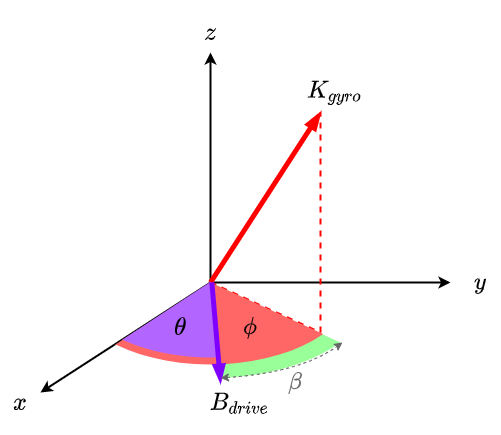
\includegraphics[width=0.5\textwidth]{Theory/Figures/NMRG_phase_dynamics.png}
\caption{NMRG phase dynamics in the lab frame of reference illustration. $\phi$ and $\theta$ are the gyro and drive phases respectively, while $\beta$ is the phase leg of the drive from the gyro.}
\label{fig:nmrg_phase_dynamics}
\end{figure}

There are few ways to use feedback in a dual-species NMRG configuration. One way is to lock the bias magnetic field to match a clock-derived NMR Xenon drive signal. We do that by keeping the gyro phase ($\phi$) locked to the NMR drive phase ($\theta$) by measuring the phase difference between the two ($\beta$) and using negative feedback to change the bias magnetic field ($B_0$) in a way that locks the phase difference to a constant value ($\beta_0$) using a PID controller following the next relation

\begin{align}
     B_{0}^{\left(t+1\right)} &= B_{0}^{\left(t\right)} - \underset{\delta B_{0}^{\left(t\right)}}{\underbrace{K_p \left[ \epsilon\left(t\right) + \frac{1}{T_i} \int_{t_i}^{t} \epsilon\left(t'\right)dt' + T_{d} \frac{d \epsilon\left(t\right)}{dt} \right]}}
\end{align}

where $T_i$ and $T_d$ are the integration and derivative times respectively. We can extract $\epsilon\left(t\right)$ from the measurement of $\beta$ following eq.(\ref{eq:phase_leg}). Another way is to use the same technique to lock the NMR drive frequency. 

\subsection{PID}
\href{https://jckantor.github.io/CBE30338/04.03-PID_Control_with_Bumpless_Transfer.html}{PID generator with python}

{\color{red} $\beta_t = \phi_t - \theta_t = \phi_t - \phi_{t-1} = \Delta \phi$}

\section{Alkali Dynamics - ESR}
The Block equation for the Alkali (Rb87) spin are given by

\begin{align}
    \frac{d \mathbf{S}}{d t} &= \gamma_{A}\left[\left( B_0 + B_1 \cos{(\omega_{1} t)}\right)\hat{z} + b_{SK} \mathbf{K}\right] \times\mathbf{S}  +\Gamma_{se} \left( \mathbf{K} - \mathbf{S}\right) - \Gamma_2 \hat{x}\left(\hat{x}\cdot \mathbf{S}\right)  - \Gamma_2 \hat{y}\left(\hat{y}\cdot \mathbf{S}\right) -  \Gamma_1 \hat{z}\left(\hat{z}\cdot \mathbf{S}\right)
\end{align}

In a matrix form

\begin{align}
    \left(\begin{matrix}
    \dot{S}_x\\
    \dot{S}_y\\
    \dot{S}_z
    \end{matrix}\right)
    &=  
    \left(\begin{matrix}
    -\Gamma_2               &  -\omega_0 - \Omega_1 \cos{(\omega_{1} t)} - \gamma_{A}b_{SK}K_z                      &  \gamma_{A}b_{SK}K_y                              \\
    \omega_0 + \Omega_1 \cos{(\omega_{1} t)}+\gamma_{A}b_{SK}K_z    &  -\Gamma_2                       &  -\gamma_{A}b_{SK}K_x \\
    -\gamma_{A}b_{SK}K_y                       &  \gamma_{A}b_{SK}K_x &  -\Gamma_1 
    \end{matrix}\right)\cdot
    \left(\begin{matrix}
    S_x\\
    S_y\\
    S_z
    \end{matrix}\right) + 
    \left(\begin{matrix}
         0  \\
         0  \\
         R_{se} 
    \end{matrix}\right)
\end{align}

thus,

\begin{align}
    \dot{S}_+ &= -\Gamma_2 S_x - \left(\omega_0 + \Omega_1 \cos{(\omega_{1} t)} + \gamma_{A}b_{SK}K_z\right) S_y + \gamma_{A}b_{SK}K_y S_z\\ &+ i\left(\omega_0 + \Omega_1 \cos{(\omega_{1} t)} + \gamma_{A}b_{SK}K_z\right) S_x -i\Gamma_2 S_y - i \gamma_{A}b_{SK}K_x S_z\\
   \dot{S}_+ &= \left[-\Gamma_2 + i\left(\omega_0 + \Omega_1 \cos{(\omega_{1} t)} + \gamma_{A}b_{SK}K_z\right) \right]S_+ - i \gamma_{A}b_{SK}\left(K_x +i K_y\right) S_z \\ 
   \dot{S}_+ &= \left[-\Gamma_2 + i\left(\omega_0 + \Omega_1 \cos{(\omega_{1} t)} + \gamma_{A}b_{SK}K_z\right) \right]S_+ - i \gamma_{A}b_{SK}K_+ S_z \\ 
\end{align}

moving to the oscillating frame of reference $S_+ = A_+ e^{i\mu_1}$, where $\mu_1 = \frac{\Omega_1}{\omega_1}\sin{\left(\omega_1 t\right)}$ we get

\begin{align}
    \dot{A}_+ e^{i\mu_1} + i\dot{\mu}_1e^{i\mu_1}A_+ &= \left[-\Gamma_2 + i\left(\omega_0 + \Omega_1 \cos{(\omega_{1} t)} + \gamma_{A}b_{SK}K_z\right) \right]A_+ e^{i\mu_1} - i \gamma_{A}b_{SK}K_+ S_z\\
    \dot{A}_+ + i\Omega_1 \cos{(\omega_{1} t)}A_+ &= \left[-\Gamma_2 + i\left(\omega_0 + \Omega_1 \cos{(\omega_{1} t)} + \gamma_{A}b_{SK}K_z\right) \right]A_+  - i \gamma_{A}b_{SK}K_+ S_z e^{-i\mu_1}\\
    \dot{A}_+  &= \left[-\Gamma_2 + i\left(\omega_0 + \gamma_{A}b_{SK}K_z\right) \right]A_+  - i \gamma_{A}b_{SK}K_+ S_z e^{-i\mu_1}\label{eq:alkali_rotating_frame}
\end{align}

we use the Jacobi–Anger expansion $e^{i z\sin{\left(\theta\right)}}=\sum_{n=-\infty}^{\infty}J_n\left(z\right)e^{i n \theta}$, using the Bessel function relation $J_{-n}(z) = (-1)^n J_n(z)$ 

\begin{align}
    e^{\pm i z\sin{\left(\theta\right)}} &= J_0\left(z\right)\pm 2i\sum_{n=0}^{\infty} J_{2n+1}\left(z\right)\sin{\left(\left(2n+1\right)\theta\right)}+2\sum_{n=1}^{\infty} J_{2n}\left(z\right)\cos{\left(2n\theta\right)} 
\end{align}

so finally


\begin{align}
        e^{-i\mu_1} = J_0\left(\frac{\Omega_1}{\omega_1}\right)+ 2i J_{1}\left(\frac{\Omega_1}{\omega_1}\right)\sin{\left(\omega_1 t\right)}+2 J_{2}\left(\frac{\Omega_1}{\omega_1}\right)\cos{\left(2\omega_1 t\right)}+\dots
\end{align}

Substituting this expansion back into eq.(\ref{eq:alkali_rotating_frame})

\begin{align}
    \dot{A}_+  &= \left[-\Gamma_2 + i\left(\omega_0 + \gamma_{A}b_{SK}K_z\right) \right]A_+ \\ &- i \gamma_{A}b_{SK}K_+ S_z \left[J_0\left(\frac{\Omega_1}{\omega_1}\right)+ 2i J_{1}\left(\frac{\Omega_1}{\omega_1}\right)\sin{\left(\omega_1 t\right)}+2 J_{2}\left(\frac{\Omega_1}{\omega_1}\right)\cos{\left(2\omega_1 t\right)}+\dots\right]
\end{align}
 
Next we would like to transform to the Fourier space so it would be easier to do so with the Jacobi–Anger expansion exponential notation, then $\mathcal{F}\left[e^{-in\omega_1 t}\right] = \sqrt{2\pi}\delta \left(\omega - n\omega_1\right)$ and

\begin{align}
    i\omega A_+\left(\omega\right)  &= \left[-\Gamma_2 + i\left(\omega_0 + \gamma_{A}b_{SK}K_z\right) \right]A_+\left(\omega\right)  - i \gamma_{A}b_{SK}K_+ S_z \sum_{n=-\infty}^{\infty}J_n\left(\frac{\Omega_1}{\omega_1}\right)\sqrt{2\pi}\delta \left(\omega + n\omega_1\right)\\
\end{align}

finally

\begin{align}
     A_+\left(\omega\right)  &= \frac{-i \gamma_{A}b_{SK}K_+ S_z}{\Gamma_2 + i\left(\omega - \omega_0 - \gamma_{A}b_{SK}K_z\right) } \sum_{n=-\infty}^{\infty}J_n\left(\frac{\Omega_1}{\omega_1}\right)\sqrt{2\pi}\delta \left(\omega + n\omega_1\right)
\end{align}

Next we swallow the $\gamma_{A}b_{SK}K_z$ term into $\omega_0$, and placing the $\frac{1}{\omega-\omega_0}$ inside the sum

\begin{align}
     A_+\left(\omega\right)  &= -i \gamma_{A}b_{SK}K_+ S_z \sum_{n=-\infty}^{\infty}J_n\left(\frac{\Omega_1}{\omega_1}\right)\sqrt{2\pi} \frac{\delta\left(\omega + n\omega_1\right)}{\Gamma_2 + i\left(\omega - \omega_0\right)}\\
      &= -i \gamma_{A}b_{SK}K_+ S_z \sum_{n=-\infty}^{\infty}J_n\left(\frac{\Omega_1}{\omega_1}\right)\sqrt{2\pi} \frac{\delta\left(\omega + n\omega_1\right)}{\Gamma_2 + i\left(n\omega_1 - \omega_0\right)}\\
      &= -\frac{i \gamma_{A}b_{SK}K_+ S_z}{\Gamma_2} \sum_{n=-\infty}^{\infty}J_n\left(\frac{\Omega_1}{\omega_1}\right)\sqrt{2\pi} \frac{\delta\left(\omega + n\omega_1\right)}{1 + i\frac{\left(n\omega_1 - \omega_0\right)}{\Gamma_2}}\label{eq:alkali_esr_frame}
\end{align}

Now, if $\omega_1-\omega_0\ll\Gamma_2\ll\omega_0$, we are left only with the $J_{-1}$ term in the sum

\begin{align}
      A_+\left(\omega\right)&= -\frac{i \gamma_{A}b_{SK}K_+ S_z}{\Gamma_2} J_{-1}\left(\frac{\Omega_1}{\omega_1}\right)\sqrt{2\pi} \delta\left(\omega - \omega_1\right)
\end{align}

back to the time domain

\begin{align}
      A_+ &= -\frac{i \gamma_{A}b_{SK}K_+ S_z}{\Gamma_2} J_{-1}\left(\frac{\Omega_1}{\omega_1}\right)e^{i\omega_1 t}
\end{align}

going back to the lab frame of reference while keeping only the $n<3$ Bessel terms in the expansion =

\begin{align}
      A_+ &= -\frac{i \gamma_{A}b_{SK}J_{-1}K_+ S_z}{\Gamma_2} e^{i\omega_1 t}\\
      S_+ &= -\frac{i \gamma_{A}b_{SK}J_{-1}K_+ S_z}{\Gamma_2}e^{i\omega_1 t}e^{i\mu_1}\\
      S_+ &= -\frac{i \gamma_{A}b_{SK}J_{-1}K_+ S_z}{\Gamma_2}e^{i\omega_1 t}\left[J_0+ 2i J_{1}\sin{\left(\omega_1 t\right)}+2 J_{2}\cos{\left(2\omega_1 t\right)}\right]
\end{align}

recall that we only care about the $S_x$ part of the transverse signal 

\begin{align}
      S_x  +i S_y &= -\frac{i \gamma_{A}b_{SK}J_{-1} S_z}{\Gamma_2}\left(K_x+i K_y\right)\left(\cos{(\omega_1 t)}+i\sin{(\omega_1 t)}\right)\left[J_0+ 2i J_{1}\sin{\left(\omega_1 t\right)}+2 J_{2}\cos{\left(2\omega_1 t\right)}\right]\label{eq:transverse_alkali_lab_frame}
\end{align}

so 

\begin{align}
      S_x &= -\frac{\gamma_{A}b_{SK}J_{-1} S_z}{\Gamma_2} \Bigg[(i)^4 2K_y J_{1}\sin{(\omega_1 t)}\sin{\left(\omega_1 t\right)}\\
      &+ (i)^2 K_y\cos{(\omega_1 t)}\left(J_0+ 2 J_{2}\cos{\left(2\omega_1 t\right)}\right)\\
      &+ (i)^2 K_x \sin{(\omega_1 t)}\left(J_0+ 2 J_{2}\cos{\left(2\omega_1 t\right)}\right)\\
      &+ (i)^2 2K_x\cos{(\omega_1 t)}J_{1}\sin{\left(\omega_1 t\right)}\Bigg]\\
      S_x &= -\frac{\gamma_{A}b_{SK}J_{-1} S_z}{\Gamma_2} \Bigg[ K_y J_{1}\left(1 - \cos{\left(2\omega_1 t\right)}\right)\\
      &-  K_y\left(J_0\cos{(\omega_1 t)}+  J_{2}\cos{(-\omega_1 t)}+J_{2}\cos{(3\omega_1 t)}\right)\\
      &-  K_x\left(J_0 \sin{(\omega_1 t)}+ J_{2} \sin{(3\omega_1 t)}+ J_{2} \sin{(-\omega_1 t)}\right)\\
      &- K_x J_{1}\left(\sin{\left(2\omega_1 t\right)}\right)\Bigg]
\end{align}

Next, assuming Lock-in detection of $S_x$ with a reference signal $\cos{\left(\omega_1 t+\alpha\right)}$, then every term which is factored with a sine / cosine function (after using trigonometric product$\to$sum identities) will be averaged out to zero, such that we are left with the next relation

\begin{align}
      \left<S_x\cos{\left(\omega_1 t+\alpha\right)}\right> &= \frac{\gamma_{A}b_{SK}J_{-1} S_z}{2\Gamma_2} \left[ K_y\cos{(\alpha)}\left(J_0+  J_{2}\right) + K_x\sin{(\alpha)}\left(-J_0 + J_{2} \right)\right]\label{eq:lockin_zero_order}
\end{align}

which is the same Lock-in relation put out in \cite{walker2016spin}. We can get a less course Lock-in relation by returning back to eq.(\ref{eq:alkali_esr_frame}) and keeping another term in the approximation, such that we take

\begin{align}
    \frac{1}{1 + i\frac{\left(n\omega_1 - \omega_0\right)}{\Gamma_2}} \approx 1 - i\frac{\left(n\omega_1 - \omega_0\right)}{\Gamma_2}
\end{align}

then, assigning eq.(\ref{eq:lockin_zero_order}) with $S_x^{(0)}$, let us calculate the additional term to $S_x=S_x^{(0)}+S_x^{(1)}$ using eq.(\ref{eq:transverse_alkali_lab_frame}))

\begin{align}
      S_x^{(1)}  +i S_y^{(1)} &= -\frac{ \gamma_{A}b_{SK}J_{-1} S_z}{\Gamma_2}\left(\frac{\left(\omega_1 - \omega_0\right)}{\Gamma_2}\right)\left(K_x+i K_y\right)\left(\cos{(\omega_1 t)}+i\sin{(\omega_1 t)}\right)\left[J_0+ 2i J_{1}\sin{\left(\omega_1 t\right)}+2 J_{2}\cos{\left(2\omega_1 t\right)}\right]
\end{align}

we need only $S_x^{(1)}$

\begin{align}
      S_x^{(1)} &= -\frac{\gamma_{A}b_{SK}J_{-1} S_z}{\Gamma_2}\left(\frac{\left(\omega_1 - \omega_0\right)}{\Gamma_2}\right) \Bigg[ (i)^2 K_y\cos{(\omega_1 t)}2 J_{1}\sin{\left(\omega_1 t\right)}\\
      &+ (i)^2 K_y \sin{(\omega_1 t)}\left(J_0+ 2 J_{2}\cos{\left(2\omega_1 t\right)}\right)\\
      &+ (i)^2 K_x \sin{(\omega_1 t)}2 J_{1}\sin{\left(\omega_1 t\right)}\\
      &+ K_x \cos{(\omega_1 t)}\left(J_0+ 2 J_{2}\cos{\left(2\omega_1 t\right)}\right)\Bigg]\\
      S_x^{(1)} &= \frac{\gamma_{A}b_{SK}J_{-1} S_z}{\Gamma_2}\left(\frac{\left(\omega_1 - \omega_0\right)}{\Gamma_2}\right) \Bigg[ 2 J_{1}K_y\cos{(\omega_1 t)}\sin{\left(\omega_1 t\right)}\\
      &+  K_y \sin{(\omega_1 t)}\left(J_0+ 2 J_{2}\cos{\left(2\omega_1 t\right)}\right)\\
      &+  2 J_{1}K_x \sin{(\omega_1 t)}\sin{\left(\omega_1 t\right)}\\
      &- K_x \cos{(\omega_1 t)}\left(J_0+ 2 J_{2}\cos{\left(2\omega_1 t\right)}\right)\Bigg]\\
      S_x^{(1)} &= \frac{\gamma_{A}b_{SK}J_{-1} S_z}{\Gamma_2}\left(\frac{\left(\omega_1 - \omega_0\right)}{\Gamma_2}\right) \Bigg[ J_{1}K_y\sin{(2\omega_1 t)}\\
      &+  K_y \left(J_0\sin{(\omega_1 t)}+ J_{2}\sin{(3\omega_1 t)}+J_{2}\sin{\left(-\omega_1 t\right)}\right)\\
      &+  J_{1}K_x \left(1 - \cos{\left(2\omega_1 t\right)}\right)\\
      &- K_x \left(J_0\cos{(\omega_1 t)}+  J_{2}\cos{(-\omega_1 t)}+ J_{2}\cos{\left(3\omega_1 t\right)}\right)\Bigg]
\end{align}

Computing the addition to the Lock-in measurement

\begin{align}
      \left<S_x^{(1)}\cos{\left(\omega_1 t+\alpha\right)}\right> &= \frac{\gamma_{A}b_{SK}J_{-1} S_z}{2\Gamma_2}\left(\frac{\left(\omega_1 - \omega_0\right)}{\Gamma_2}\right) \left[K_y\sin{(\alpha)} \left(-J_0+J_{2}\right)- K_x \cos{(\alpha)}\left(J_0+  J_{2}\right)\right]
\end{align}

finally, putting all together 

\begin{align}
      \left<\left(S_x^{(0)}+S_x^{(1)}\right)\cos{\left(\omega_1 t+\alpha\right)}\right> &= \frac{\gamma_{A}b_{SK}J_{-1} S_z}{2\Gamma_2} \bigg[\left(K_x + K_y \frac{\left(\omega_1 - \omega_0\right)}{\Gamma_2}\right)\sin{(\alpha)}\left(-J_0+J_{2}\right) \\
      &+ \left(K_y- K_x\frac{\left(\omega_1 - \omega_0\right)}{\Gamma_2}\right) \cos{(\alpha)}\left(J_0+  J_{2}\right)\bigg]\label{eq:lockin_zero_first_order_sx}
\end{align}

In an on resonance working point $\omega_1=\omega_0$, and the measured signal would be

\begin{align}
      \left<\left(S_x^{(0)}+S_x^{(1)}\right)\cos{\left(\omega_1 t+\alpha\right)}\right> &= \frac{\gamma_{A}b_{SK}J_{0}J_{-1} S_z}{\Gamma_2} K_y \cos{(\alpha)}
\end{align}

\section{Balanced Photo Diode}

% Now, assume $\omega_0 \gg \Gamma_2^A$ then 

% in steady state

% \begin{align}
%     A_+  &= \frac{i \gamma_{A}b_{SK}K_+ S_z}{\Gamma_2 + i\left(\omega_0 + \gamma_{A}b_{SK}K_z\right)} e^{i\mu_1}
% \end{align}



\bibliographystyle{alpha}
\bibliography{my_bib}

\end{document}
